\chapter{慢扫描电视}

{\em 慢扫描电视 (SSTV)} 是用于传输图像的一种通信模式. 慢扫描电视是一种窄带通信, 它可以用从单边带 (SSB) 电台的音频通道发射到业余频段上. 在传播良好的情况下, 高频段的世界范围的通信也是可能的. 

\section{起源}

在1957年, 一名肯塔基大学的学生Copthorne "Cop" Macdonald, WA2BCW (现VY2CM), 发现了一篇论文, 讲述了用贝尔实验室发明的设备在电话线上传输图像. 这个通信系统让这位业余无线电爱好者着迷, 因为它需要的带宽和话音一样窄, 而且能够用一般的业余无线电台传输. 

在当时另一种图像模式无线电传真(Facsimile)是可用的, 但是它需要更长的时间 (约 20 分钟) 来传送高清晰度的图像. 这样的持续时长不能在一次QSO中提供时间一致性, 并且需要一台复杂的机械打印机和电敏纸. 有必要发明另一种方式. 

有一种想法是将要传输的图像编码到音频信号中, 并显示在长余辉显示器(用于雷达或慢扫描示波器的显像管)上. 

然后 Copthorne 开始研究怎样将图像通过业余收发信机在无线电波传输. 他在六个月内做了许多关于调频和调谐的实验, 慢扫描电视的设计就从中诞生. 接下来的六个月他制造了一台 SSTV 图像扫描仪, 这样实验就能在业余频段开展了. 在1959年12月20日, 第一张电视图像跨越了大西洋. 

\begin{figure}
	\centering
	\subfigure[第一张跨越大西洋的图像, 由John Plowman G3AST接收]{
		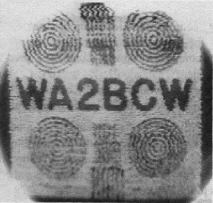
\includegraphics[width=0.45\linewidth]{figs/obrazek1.png}}
	\subfigure[Copthorne Macdonald 正在播报]{
		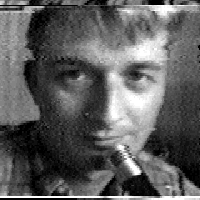
\includegraphics[width=0.45\linewidth]{figs/copthorn.png}}
	\caption{早期 SSTV 图像}
\end{figure}
	
在接下来的十年里 Copthorne 和一群业余爱好者继续改进 SSTV, 他们建立了基本的SSTV标准并开发了一种取样相机. 他们的工作于1968年完成. 美国联邦通信委员会 (FCC) 正式授权了SSTV操作. 

几个月后业余无线电杂志刊登了第一篇关于这种新通信模式的文章. 这篇文章引发了火腿们极大的兴趣和一个真正的 SSTV 热潮. 

\section{图像传输}

SSTV 的基本思想是使用标准收发信机传输电视图像. 然而, 电视广播需要更宽的频宽, 电视信号的缩减需要靠降低水平 (行) 和垂直 (帧) 扫描的次数来实现, 且必须缩减到最少的频率. 这就意味着一个典型的黑白电视信号必须从 3 MHz 频宽缩减到 3 kHz --- 缩减率接近 1000:1. 如今频宽缩减更加严重, 因为彩色电视图像需要将近 6 MHz 的频宽. 由于巨大的频宽缩减, 只有低清晰度的静止图像才能被传输. 

在实验中, 我们发现图像可以在带有 P7 磷光体的长余辉显像管上保持可见约 8 秒. 所以在接收完最后一行后, 第一行依然可见, 但在一段时间内会慢慢消失. 为了达到最佳效果, 需要在黑暗的房间里观看SSTV显示器. 通常几个相同的图像会一次传输, 每个后续图像会缓慢地将原始图像还原在磷光体上, 原始图像依然可见. 这样就允许图像显示更长的时间或录像以供之后回放. 

我们发现电子电路正确检测出行同步脉冲的理想时间是5毫秒, 检测出帧(垂直)同步脉冲的理想时间是30毫秒. 帧同步开启显像管图像显示的自动启动. 

扫描线和帧的同步频率是从电源频率推导出的. 水平扫描的频率是 $50 Hz / 3 = 16.6 Hz$, 垂直扫描的频率是 $1/7.2 s=0.1388 Hz$, 这是由电源频率除以 360 (3 $\times$ 120 行) 得出的. 在电源频率是 60 Hz 的国家, 这些频率的推导方法相同. 

视频信号的频带的选择范围在 1500 Hz 为黑色, 2300 Hz 为白色之间. 同步脉冲在 1200 Hz 频率上, 因为它比“黑色信号还要黑”, 所以不会影响图像信息. 所有SSTV频率分量都在低频带内, 可以通过语音频道传输. 

从这个原始标准产生的其他SSTV模式, 它们绝大部分都只在扫描速度和彩色传输的增加方面不同. 
